\chapter{評価}
\label{evaluation}

本章では第4章の\ref{implementation}で設定した3つの実験の結果及び考察を行う。

実験1の結果\label{evo1}では\ref{exp1}で示した設定もとに実験を行い、その結果を述べ各データセットにおいてどの程度の学習性能を示したか結論を述べる。
実験2の結果\label{evo2}では\ref{exp2}で示した設定もとに実験を行い、\ref{af-class}の表を軸にどのような活性化関数になったか、損失を見ながら考察を行い結論を述べる。
実験3の結果\label{evo3}では\ref{exp3}で示した設定もとに実験を行い、一般的にどのような条件でK-AFがより良い性能を出すか、また、欠点が存在するか調査する。

\label{result}では各実験による考察結果から、\ref{kadai}に対してどの程度K-AFが性能を示すことができたか分析を行う。
そして最後に第6章への結論\ref{conclusion}へと導く。


\section{実験1の結果 既存の活性化関数との比較実験}
\label{evo1}
\ref{exp1}で示した比較実験の結果を記述する。

\subsection{irisでの比較実験}
\label{ev:iris}

第4章の\ref{impl:iris}で設定した実験を行い、結果を以下にまとめた。
\subsubsection{設定1及び設定2の結果と考察}


\begin{table}[htbp]
    \begin{center}
        \caption{irisの設定1及び設定2のAccuracy}
        \vspace{2mm} 
        \begin{tabular}{l*{2}{c}r}
            活性化関数  & 設定1のAccuracy &  設定2のAccuracy \\
            \hline
            K-AF            & 0.0 & 0.0 \\
            Sigmoid            & -22.0 & 0.0\\
            Linear            & 0.0 & 0.0\\
            ReLU        & -22.0 & 0.0\\
            Swish           & 0.0 & 0.0 \\
            Mish           & -1.0 & 0.0\\
    
        \end{tabular}
    \end{center}
\end{table}



irisでは十分な性能を出すことができた。


\subsection{digitsでの比較実験}
\label{ev:digitsでの比較実験}
第4章の\ref{impl:digits}で設定した実験を行い、結果を以下にまとめた。
\subsubsection{設定1及び設定2の結果}
\label{digits:result}

\begin{table}[htbp]
    \begin{center}
        \caption{digitsの設定1及び設定2のAccuracy}
        \vspace{2mm} 
        \begin{tabular}{l*{2}{c}r}
            活性化関数              & 設定1のAccuracy &  設定2のAccuracy \\
            \hline
            K-AF            & 91.6 & 60.0 \\
            Sigmoid            & 92.0 & 68.6\\
            Tanh            & 95.6 & 89.6 \\
            ReLU        & 38.0 & 54.3 \\
            Swish           & 50.3 & 56.6 \\
            Mish           & 55.6 & 53.3 \\
    
        \end{tabular}
    \end{center}
\end{table}


\subsubsection{設定1及び設定2のLossTrainig}
\label{digits:loss}



\begin{figure}[hbtp]
    \begin{center}
        \begin{tabular}{c}
            \begin{minipage}{0.5\hsize}
                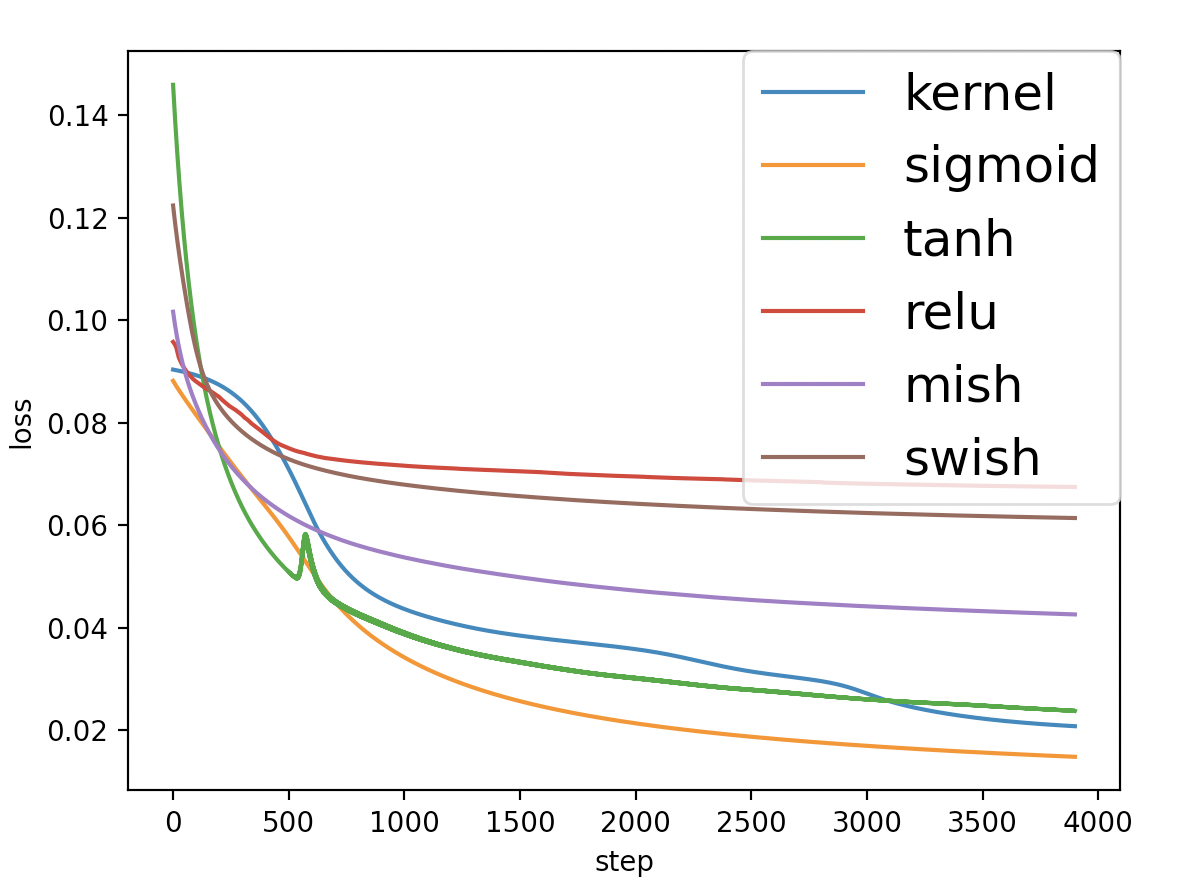
\includegraphics[clip, width=7cm]{asset/digits_0.01_4000_3_002_sgd_non_kaiming_uniform.png}
                    \caption{digitsの設定1の結果のLossTraining}
                    \label{digits_1}
            \end{minipage}
            \hspace{10pt}
            \begin{minipage}{0.5\hsize}
                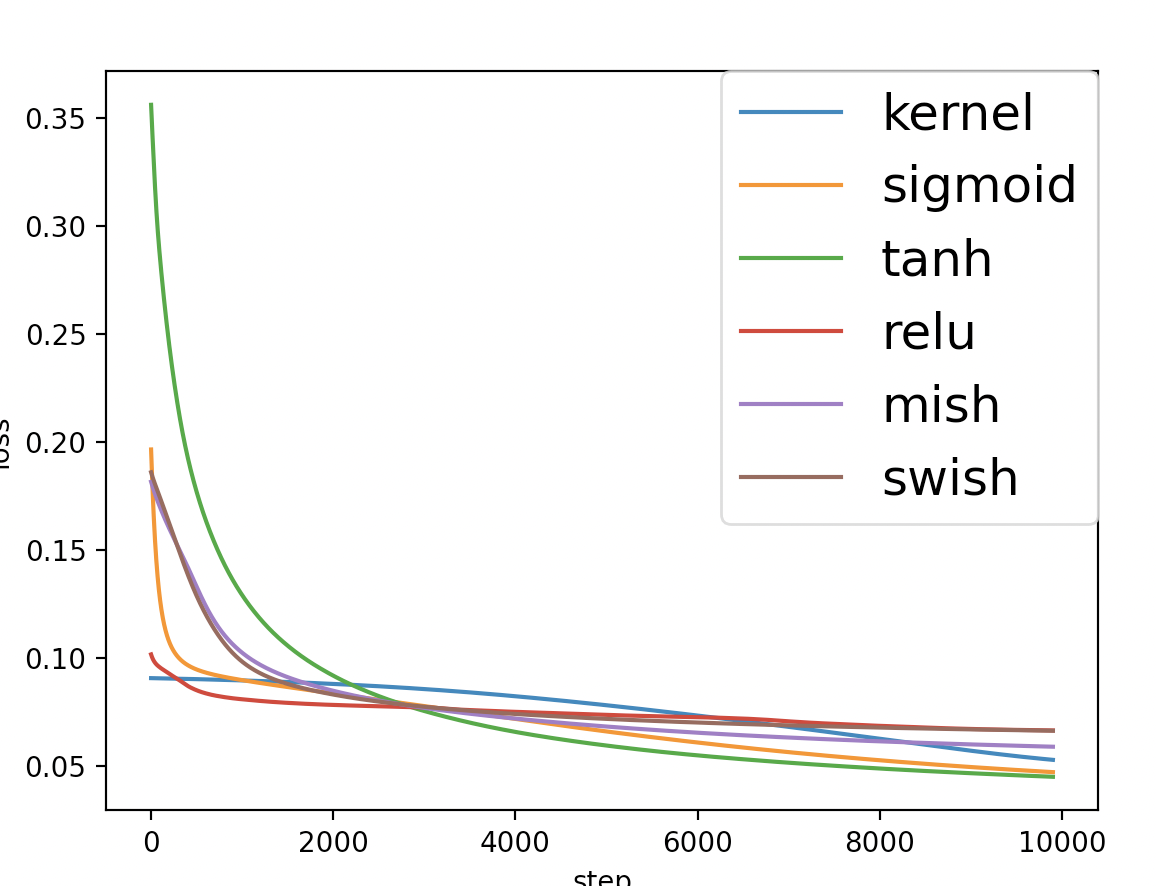
\includegraphics[clip, width=7cm]{asset/digits_0.001_10000_3_002_sgd_non_kaiming_uniform.png}
                    \caption{digitsの設定2の結果のLossTraining}
                    \label{digits_2}
            \end{minipage}
        \end{tabular}
    \end{center}
\end{figure}


\subsubsection{digitsでの実験結果の考察}
結果\ref{digits:result}を見ると設定1の場合では91.6%とSigmoidやTanhといったラベリングによく用いられる活性化関数に匹敵する精度を出せた。ReLU、Mish、Swish等のの上限値が存在しない関数よりも遥かに良い性能を出すことができた。
設定2の場合でもSigmoidやTanhほどの成果は出なかったものの、上限値が存在しない関数よりはいい性能を出すことができた。

TrainigLossのグラフ\ref{digits:result}を見ると、設定の1,2共に順調に下に推移してることがわかる。



\subsection{wineでの実験と設定}
\label{ev:wineでの実験と設定}

\subsubsection{設定1及び設定2の結果と考察}


\begin{table}[htbp]
    \begin{center}
        \caption{wineの設定1及び設定2の結果Accuracy}
        \vspace{2mm} 
        \begin{tabular}{l*{2}{c}r}
            活性化関数              & 設定1のAccuracy &  設定2のAccuracy \\
            \hline
            K-AF            & 0.0 & 0.0 \\
            Sigmoid            & -22.0 & 0.0\\
            Linear            & 0.0 & 0.0\\
            ReLU        & -22.0 & 0.0\\
            Swish           & 0.0 & 0.0 \\
            Mish           & -1.0 & 0.0\\
    
        \end{tabular}
    \end{center}
\end{table}



irisでは十分な性能を出すことができた。


\subsection{bostonでの比較実験}
\label{ev:bostonでの比較実験}

\subsubsection{設定1及び設定2の結果と考察}


\begin{table}[htbp]
    \begin{center}
        \caption{bostonの設定1及び設定2のAccuracy}
        \vspace{2mm} 
        \begin{tabular}{l*{2}{c}r}
            活性化関数              & 設定1のAccuracy &  設定2のAccuracy \\
            \hline
            K-AF            & 0.0 & 0.0 \\
            Sigmoid            & -22.0 & 0.0\\
            Linear            & 0.0 & 0.0\\
            ReLU        & -22.0 & 0.0\\
            Swish           & 0.0 & 0.0 \\
            Mish           & -1.0 & 0.0\\
    
        \end{tabular}
    \end{center}
\end{table}



irisでは十分な性能を出すことができた。



\subsection{breast\_cancerでの比較実験}
\label{ev:breastcancer}

\subsubsection{設定1及び設定2の結果と考察}


\begin{table}[htbp]
    \begin{center}
        \caption{breast\_cancerの設定1及び設定2のAccuracy}
        \vspace{2mm} 
        \begin{tabular}{l*{2}{c}r}
            活性化関数              & 設定1のAccuracy &  設定2のAccuracy \\
            \hline
            K-AF            & 0.0 & 0.0 \\
            Sigmoid            & -22.0 & 0.0\\
            Linear            & 0.0 & 0.0\\
            ReLU        & -22.0 & 0.0\\
            Swish           & 0.0 & 0.0 \\
            Mish           & -1.0 & 0.0\\
    
        \end{tabular}
    \end{center}
\end{table}



irisでは十分な性能を出すことができた。



\subsection{実験1全体のまとめ}
結果全体を見ると、K-AFは高いLearningRateに対してもロバストに学習を行うことができる。



\section{実験2の結果 K-AFの関数形状の調査}
\label{evo2}
\ref{exp2}で示した比較実験の結果を記述する。


\begin{figure}[hbtp]
    \begin{center}
        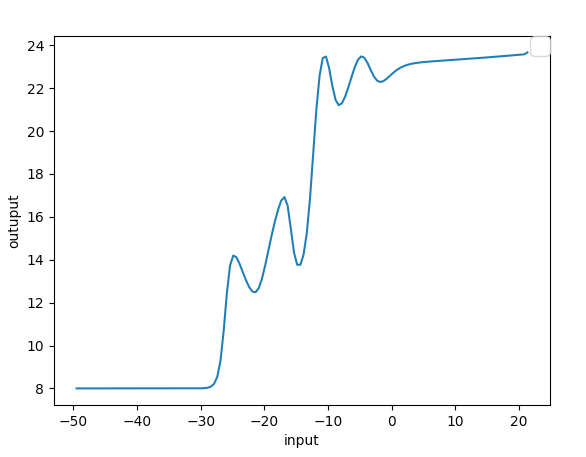
\includegraphics[width=10cm]{asset/boston_0000001_SGDkaiming_normal__non_200_function_2.png}
            \caption{活性化関数の形}
            \label{boston}
    \end{center}
\end{figure}


\section{実験3の結果 K-AFの性能が上がる条件探査}
\label{evo3}
\ref{exp3}で示した比較実験の結果を記述する。
wine及びbostonのデータセットで最も性能が良かったニューラルネットワークの設定のトップ5を記述する。

\subsubsection{wineの場合}

\begin{table}[htbp]
    \begin{center}
        \caption{wineを推論するときの最もいい設定}
        \label{winebest}
        \vspace{2mm} 
        \begin{tabular}{ |c|c|c| }
        組み合わせ & Acc & エラーの回数 \\
        \hline
        iris           & $ 10^{-3} $    & 3 \\
        digits         & $ 10^{-3} $    & 3 \\
        wine           & $ 10^{-3} $    & 3 \\
        boston         & $ 10^{-3} $    & 13  \\
        breast\_cancer & $ 10^{-3} $    & 30 \\
        \end{tabular}
    \end{center}
\end{table}

表\ref{winebest}を参考にすると

\subsubsection{bostonの場合}

\begin{table}[htbp]
    \begin{center}
        \caption{bostonを推論するときの最もいい設定}
        \label{bostonbest}
        \vspace{2mm} 
        \begin{tabular}{ |c|c|c| }
        組み合わせ & Acc & エラーの回数 \\
        \hline
        iris           & $ 10^{-3} $    & 3 \\
        digits         & $ 10^{-3} $    & 3 \\
        wine           & $ 10^{-3} $    & 3 \\
        boston         & $ 10^{-3} $    & 13  \\
        breast\_cancer & $ 10^{-3} $    & 30 \\
        \end{tabular}
    \end{center}
\end{table}




\subsection{性能評価まとめ}
wineとbostonの結果をまとめるとと言うことがわかった。


\section{まとめ}

K-AFの精度、勾配消失の有無、実用性の観点から先行研究との比較を行った。
実験結果を踏まえ, 第 6 章で解決した課題をまとめ、将来への展望を述べる。


%%% Local Variables:
%%% mode: japanese-latex
%%% TeX-master: "./thesis"
%%% End:
